\documentclass{beamer}
\usepackage[utf8]{inputenc}
\usepackage{hyperref}
\usepackage{multicol}
\usepackage{hyperref}
\usepackage{amsmath}
\usepackage[english]{babel}
\usepackage{algorithm}
\usepackage[noend]{algpseudocode}

\inputencoding{utf8}

\mode<presentation> {
    \usetheme{Madrid}
}

\usepackage{graphicx}
\usepackage{booktabs}

\title[Heap]{Heaps}
\author{Ernesto Rodriguez - Juan Roberto Alvaro Saravia}
\institute{
    Universidad Francisco Marroquin \\
    \medskip \textit{ernestorodriguez@ufm.edu - juanalvarado@ufm.edu}
}

\date[\today]{}

\begin{document}

\begin{frame}
\titlepage
\end{frame}

\begin{frame}
\frametitle{Heap Binario}
\begin{itemize}
    \item{Se puede representar con un arreglo}
    \item{Cada elemento del arreglo es un nodo del heap}
    \item{Todo elemento (menos el primero) tiene un padre}
    \item{Todo elemento tiene como maximo dos hijos: derecho e izquierdo}
    \item{Existe una porpiedad $p$, tal que:
    \[
        \forall\ n_i\in Ns.\ p\ (\mathtt{padre}\ n_i)\ n_i
    \]}
    \item{La propiedad $p$ define un orden: $p\ a\ b\ \&\ p\ b\ c\rightarrow\ p\ a\ c$}
    \item{Cuando un heap se representa con un arreglo:
    \[
        \begin{array}{l}
            \mathtt{padre}\ n_i:=n_{i/2} \\
            \mathtt{hijo\_izquierdo}\ n_i:=n_{2i}\\
            \mathtt{hijo\_derecho}\ n_i:=n_{2i+1}
        \end{array}
    \]
    }
\end{itemize}
\end{frame}

\begin{frame}
\frametitle{Heap Binario}
Si $p\ a\ b:=\ a\geq b$
\\
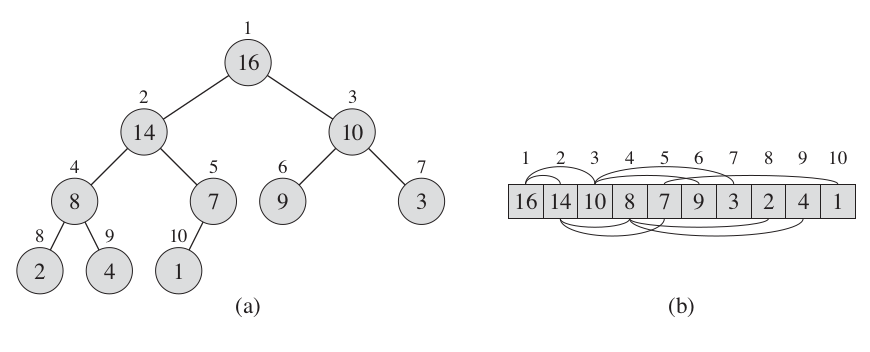
\includegraphics[width=12cm]{bheap.png}
\end{frame}

\begin{frame}
    \frametitle{Min y Max Heap}
    \begin{itemize}
        \item{En este curso se consideraran dos heaps:
        \begin{itemize}
            \item{Cuando (max heap) $p\ a\ b:=\ a\geq b$}
            \item{Cuando (min heap) $p\ a\ b:=\ a\leq b$}
        \end{itemize}
        }
        \item{¿Que valor seria la raiz en un min y max heap?}
        \item{¿Que caracteristica cumplen los hijos de todo valor?}
        \item{Los algoritmos de ordenamiento por lo general utilizan el max heap}
        \item{Un min heap se utiliza a menudo para colas}
        \item{{\bf Nota:} A partir de este momento, la palabra heap se
        referira a un max heap.}
    \end{itemize}
\end{frame}

\begin{frame}
    \frametitle{La invariante de heaps}
    \begin{itemize}
        \item{¿Que propiedades se cumplen para todo heap?}

    \end{itemize}
\end{frame}

\begin{frame}
    \frametitle{La invariante de (max) heaps}
    \begin{itemize}
        \item{¿Que propiedades se cumplen para todo heap?
        \begin{enumerate}
            \item{$\forall\ n_i\in Ns.\ \mathtt{padre}\ n_i\geq n_i$}
            \item{$\forall\ n_i\in Ns.\ \mathtt{hijo\_derecho}\ n_i\leq n_i$}
            \item{$\forall\ n_i\in Ns.\ \mathtt{hijo\_izquierdo}\ n_i\leq n_i$}
        \end{enumerate}
        \item{Se utilizara la primera (1) como la invariante. Tambien se
        llamara la ``Condicion de un heap''.}
        }
    \end{itemize}
\end{frame}

\begin{frame}
    \frametitle{Heapify}
    \begin{itemize}
        \item{Algoritmo que restaura la condicion de un heap.}
        \item{Funciona inductivamente:
        \begin{itemize}
            \item{Dado un elemento $n_i$, asumir que los heaps
            encabezados por ``$\mathtt{hijo\_derecho}\ n_i$'' e ``$\mathtt{hijo\_izquierdo}\ n_i$''
            son un heap y cumplen la condici\'on de heap.}
        \end{itemize}}
    \end{itemize}
\end{frame}

\begin{frame}
    \frametitle{Heapify}
    \begin{itemize}
        \item{Algoritmo que restaura la condicion de un heap.}
        \item{Funciona inductivamente:
        \begin{itemize}
            \item{Dado un elemento $n_i$, asumir que los heaps
            encabezados por ``$\mathtt{hijo\_derecho}\ n_i$'' e ``$\mathtt{hijo\_izquierdo}\ n_i$''
            son un heap y cumplen la condici\'on de heap.}
            \item{Si $n_i < \mathtt{hijo\_derecho}\ n_i$ o $n_i < \mathtt{hijo\_izquierdo}$,
            intercambiar el mayor de estos valores con $n_i$}
            \item{Repetir el algoritmo con el valor que fue intercambiado.}
        \end{itemize}}
    \end{itemize}
\end{frame}

\begin{frame}

    \frametitle{Heapify}

    \begin{algorithm}[H]
        \caption{Heapify}
        \begin{algorithmic}[1]
        \Procedure{heapify}{$Ns$,$i$}
        \State $izq\gets\mathtt{hijo\_izquierdo}(i)$
        \State $der\gets\mathtt{hijo\_derecho}(i)$
        \State $mayor\gets i$
        \If{$izq\leq\mathtt{len}(Ns)$ and $Ns[izq]>Ns[mayor]$}
            \State $mayor\gets izq$
        \EndIf
        \If{$der\leq\mathtt{len}(Ns)$ and $Ns[der]>Ns[mayor]$}
            \State $mayor\gets der$
        \EndIf
        \If{$mayor\neq i$}
            \State $\mathtt{intercambiar}(Ns,i,mayor)$
            \State $\mathtt{heapify}(Ns, mayor)$
        \EndIf
        \EndProcedure
        \end{algorithmic}
    \end{algorithm}
    
\end{frame}

\end{document}